\documentclass[main.tex]{subfiles}
\begin{document}

\title{
    \textbf{Algorytmy ewolucyjne i metaheurystyki}\\
    \begin{large}
        Sprawozdanie 6
    \end{large}
}

\author{
    Górka Bartosz\\
  \texttt{127228}
  \and
  Zimniak Kajetan\\
  \texttt{127229}
}

\date{}

\maketitle

\section{Opis etapu projektu}
Celem kolejnego etapu projektu było zaimplementowanie \texttt{hybrydowego algorytmu ewolucyjnego} wraz z operatorem rekombinacji i porównanie wyników do metod \texttt{Multiple start local search} oraz \texttt{Iterated local search} stworzonych i opisanych w poprzednich etapach projektu.

Liczba grup, funkcja celu oraz instancja testowa pozostały niezmienne.
Ograniczenie czasowe nowego algorytmu (podobnie jak dla ILS) ustalone zostało na czas trwania jednej iteracji algorytmu MSLS.

Algorytm hybrydowy w każdym swoim przejściu wybiera 15-elementową populację z wykorzystaniem selekcji elitarnej bez powtórzeń. Porównanie i wybór dwóch najlepszych rozwiązań odbywa się poprzez sprawdzenie wartości funkcji celu.

Rozwiązania są następnie rekombinowane, oraz przy pomocy lokalnego przeszukiwania w wersji zachłannej wstawiane do rozwiązania. Wykorzystano tę samą wersję lokalnego przeszukiwania co w przypadku porównywanych algorytmów. Rozwiązanie startowe jest losowane.

W rozdziale \ref{section:pseudokody} zaprezentowano pseudokod stworzonego algorytmu, w rozdziale \ref{section:wyniki} wyniki działania i porównanie z metodami MSLS i ILS z dużą perturbacją. Ostatni rozdział dotyczy wizualizacji uzyskanych wyników dla \texttt{hybrydowego algorytmu ewolucyjnego}.

\section{Pseudokod}
\label{section:pseudokody}
\subsection{Algorytm hybrydowy}
\begin{verbatim}
Wykonuj aż utworzysz 15-elementową populację startową {
    Zainicjalizuj losowy przydział punktów do grup
    Uruchom algorytm lokalnego przeszukiwania w wersji zachłannej
    Jeżeli rozwiązanie nie istnieje w populacji {
        Dodaj rozwiązanie do populacji
    }
}

W pętli wykonaj iteracje aż osiągniesz limit czasowy wyznaczony
przez jedną iterację MSLS {
    Wybierz losowo 2 różnych rodziców
    Dokonaj rekombinacji
    Uruchom algorytm lokalnego przeszukiwania w wersji zachłannej
        na zrekombinowanym rozwiązaniu
    Zastosuj selekcję elitarną i dodaj rozwiązanie do populacji
        jeżeli w niej nie istnieje
}
\end{verbatim}
Algorytm wykorzystuje metodę rekombinacji. Jej dokładna realizacja została przedstawiona w kolejnym punkcie.

\subsection{Rekombinacja}
\begin{verbatim}
Wyznacz zbiory punktów, które znajdują się w tych samych grupach w obu rodzicach.

Utwórz bazowe rozwiązanie na podstawie wyznaczonych zbiorów.

Wykonuj dopóki istnieją nieprzydzielone do żadnej grupy punkty {
    W sposób losowy wyznacz numer grupy
    Dodaj punkt do wyznaczonej grupy
}
\end{verbatim}

\section{Wyniki eksperymentów obliczeniowych}
\label{section:wyniki}

W tabeli \ref{table:wyniki} zaprezentowano wyniki eksperymentów obliczeniowych. Dokonano $10$ powtórzeń obliczeń.

\begin{table}[H]
\centering
\caption{Wyniki eksperymentów obliczeniowych}
\label{table:wyniki}
\resizebox{\textwidth}{!}{%
\begin{tabular}{|c|r|r|r|r|}
\hline
\textbf{Cecha} &                                                        \multicolumn{1}{c|}{\textbf{MSLS}} &  \multicolumn{1}{c|}{\textbf{ILS big perturbation}} &
\multicolumn{1}{c|}{\textbf{Evolutionary algorithm}}

                                       \\ \hline
\textbf{\begin{tabular}[c]{@{}c@{}}Wartość maksymalna\\funkcji celu\end{tabular}}
&   26.386
&   26.610
&   26.379\\ \hline
\textbf{\begin{tabular}[c]{@{}c@{}}Wartość średnia\\funkcji celu\end{tabular}}
&   26.375
&   26.407
&   26.373                                                \\ \hline
\textbf{\begin{tabular}[c]{@{}c@{}}Wartość minimalna\\funkcji celu\end{tabular}}
&   26.370
&   26.388
&   26.365                                                \\ \hline

\end{tabular}%
}
\end{table}
Algorytm ILS wykonał średnio 1250 iteracji, natomiast hybrydowy algorytm ewolucyjny 140 w czasie jednej iteracji MSLS.
Jednakże algorytm stworzony na tym etapie projektu okazał się najlepszym z dotychczas testowanych.


\section{Wizualizacja najlepszych rozwiązań}
W rozdziale zaprezentowano wizualizację najlepszego uzyskanego rozwiązania przydziału punktów do grup dla hybrydowego algorytmu ewolucyjnego.

\begin{figure}[H]
     \begin{center}
        \subfigure{
            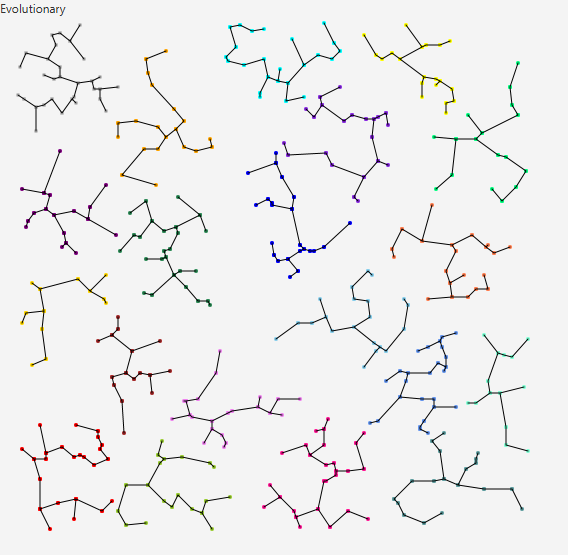
\includegraphics[width=0.45\textwidth]{sprawozdanie_6/evolutionary1.PNG}
        }
        \subfigure{
           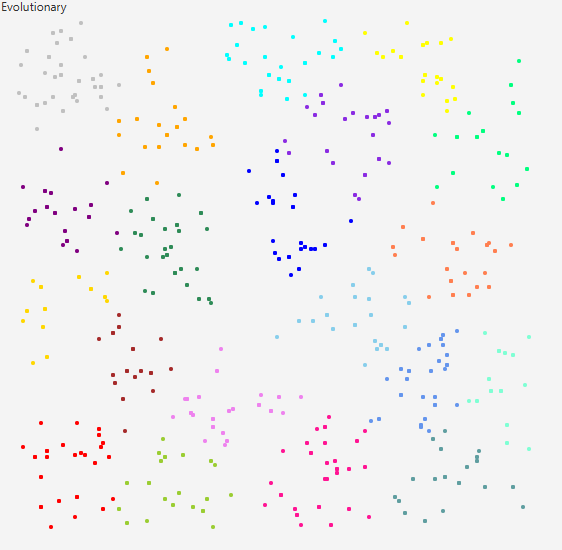
\includegraphics[width=0.45\textwidth]{sprawozdanie_6/evolutionary2.PNG}
        }\\
        \subfigure{
            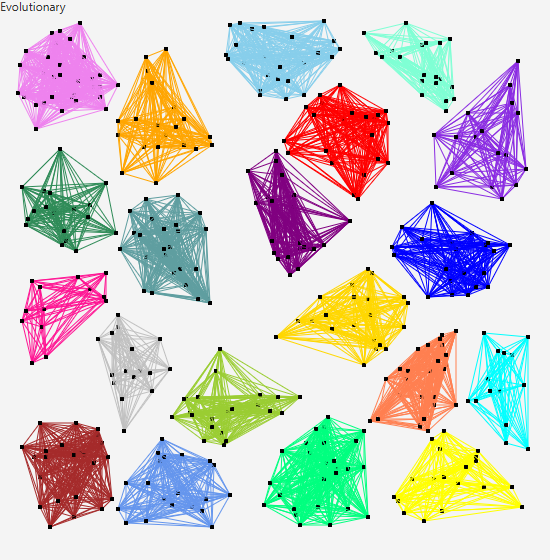
\includegraphics[width=0.45\textwidth]{sprawozdanie_6/evolutionary3.PNG}
        }
    \end{center}
\end{figure}


\end{document}
